\documentclass[11pt,letterpaper]{article}

\author{Jacob Thomas Errington}
\title{Assignment \#1\\Program Analysis \& Transformations}
\date{6 October 2016}

\usepackage[margin=2.0cm]{geometry}
\usepackage{amsmath,amssymb,amsthm}
\usepackage{tikz}
\usepackage{tikz-qtree}
\usepackage{listings}

\DeclareMathOperator{\inputOp}{in}
\DeclareMathOperator{\outputOp}{out}
\DeclareMathOperator{\killOp}{kill}
\DeclareMathOperator{\genOp}{gen}
\newcommand{\In}[1]{\inputOp{(#1)}}
\newcommand{\Out}[1]{\outputOp{(#1)}}
\newcommand{\Kill}[1]{\killOp{(#1)}}
\newcommand{\Gen}[1]{\genOp{(#1)}}

\newcommand{\intty}{\mathtt{int}}
\newcommand{\doublety}{\mathtt{double}}
\newcommand{\arrayty}{\mathtt{array}}

\usetikzlibrary{arrows,automata,positioning}

\newcommand{\matlab}{\textsc{Matlab}}

\lstset{
    basicstyle=\ttfamily
}

\begin{document}

\maketitle

\section{Background}

The program we have chosen to benchmark is an implementation of an $n$-body
simulation.  The key property of an $n$-body system is that it consists of $n$
distinct parts -- the bodies -- which act independently on all of each other.
The system is generally held to the assumption that the bodies do not collide,
and that they are points (i.e. they have no volume). In a gravitational
$n$-body system, each \emph{planet} acts on each other planet in a pairwise
fashion according to the laws of gravity. Our program simulates an $n$-body
Newtonian gravitational system.

$n$-body simulations are interesting for several reasons. In physics, many
problems can be modelled as $n$-body problems, sometimes with very large $n$.
For example, the solar system is an $n$-body system. (However, The solar system
is a somewhat uninteresting $n$-body system because the sun dominates the
system. It is usually possible to neglect the action of the other bodies
without loss of much precision, and instead study several 2-body systems.)
Other systems in which many particles interact can be modelled similarly, such
a systems of subatomic particles, provided that the inter-particle interactions
are pairwise. In specifically gravitational systems, it is possible to find a
closed, analytic solution for $n = 2$ and for special situations when $n = 3$,
but there is no general analytic solution otherwise. Hence, our simulation uses
numerical methods to find the solution. More specifically, our solution is
obtained by numerically solving differential equations. Many other problems in
science are solved by numerically solving systems of differential equations, so
looking into the optimiation of these numerical solutions can have many
practical outcomes.

From the perspective of a compiler optimizer, the numerical integration method
that we implemented is straightforward, but exhibits a number of interesting
properties. Specifically, there is a nested loop, a few auxiliary functions,
floating-point arithmetic, and many vector operations.

\section{Data}

\subsection{Running the benchmark}

Our simulation can be run by invoking the \texttt{runner} function with the
desired value of $n$ and the amount of time to run the simulation for. This
amount of time is not a \emph{real} number of sections, but rather a number of
seconds \emph{in the system}. Due to the pairwise operation of the laws of
physics, and the fact that we have used a straightforward naive implementation
without any approximations, the main algorithm has quadratic runtime in the
number of bodies, and a linear runtime in the amount of time simulated.

\subsection{First results}

\begin{figure}[ht]
    \centering
    \begin{tabular}{|c|}
        \hline
        \textbf{Runtime (s)} \\ \hline \hline
        6.8777 \\
        7.0278 \\
        6.9381 \\
        7.1604 \\
        6.9999 \\
        6.9287 \\
        6.9442 \\
        6.9730 \\
        7.0078 \\
        6.9989 \\ \hline
    \end{tabular}

    \caption{
        Some runtimes for the simulation. We ran the simulation with fifteen
        bodies in the system with randomly generated positions and momenta. The
        system was simulated for two seconds, with a time step of $0.001$
        giving $2000$ iterations per run.
        Minimum runtime: $6.8777$.
        Maximum runtime: $7.1604$.
        Average runtime: $6.9857$ (standard deviation $0.0762$).
    }
    \label{data:unoptimized-run}
\end{figure}

Figure \ref{data:unoptimized-run} shows ten runs of the simulation with
identical parameters. Although the starting conditions of the simulation are
randomized, we seed the random number generator with the same value in order to
ensure determinism of the results. This data was obtained using \matlab{} r2015a
on a laptop running Arch Linux, kernel version 4.4.19, with a (dual-core) Intel
Celeron 2957U processor $1.40 \text{GHz}$.

\section{Aspect\matlab{}}

The program we are benchmarking makes use of three very important arrays:
\begin{enumerate}
    \item
        \texttt{X} tracks the current position of each of the bodies.
    \item
        \texttt{P} tracks the current momentum of each of the bodies.
    \item
        \texttt{M} holds the mass of each of the bodies. This quantity does not
        change.
\end{enumerate}

It could be interesting to track reads and writes to each of these arrays, so
we wrote an Aspect\matlab{} aspect to do just that. One would expect read and
write counts to be proportional to the number of iterations performed by the
simulation.

\subsection{Remarks on running the woven code}

The introduction of the aspect \emph{substantially} slowed down the execution
of the benchmark. And by \emph{substantially}, I mean \emph{seriously
considerably really a lot}. Looking at the woven code reveals why: a tremedous
number of temporary variables are introduced by Aspect\matlab{}! I believe this
to be the primary cause of the slowdown. In almost all cases, these temporaries
serve no purpose in the woven code. Certainly, they are useful for other types
of pointcuts, but for those that we used in our aspect.

This suggests a number of optimization opportunities in the Aspect\matlab{}
compiler!

\subsection{Data}

\begin{figure}[ht]
    \centering
    \begin{tabular}{|c|}
        \hline
        \textbf{Runtime (s)} \\ \hline \hline
        201.9215 \\
        203.2561 \\
        216.6258 \\
        222.9545 \\
        201.9432 \\
        203.7011 \\
        201.5871 \\
        201.4031 \\
        202.5537 \\
        202.9298 \\ \hline
    \end{tabular}

    \caption{
        We ran the woven code produced by the Aspect\matlab{} compiler with the
        exact same configuration as the unwoven code used to produce that data
        in figure \ref{data:unoptimized-run}.
        Minimum runtime: $201.4031$.
        Maximum runtime: $222.9545$.
        Average runtime: $205.8876$ (standard deviation $7.5133$).
    }
    \label{fig:wovenrun}
\end{figure}

As we can see in figure \ref{fig:wovenrun}, the runtimes are substantially
increased, due to the overhead introduced by the Aspect\matlab{} compiler

\section{Using the \matlab{} profiler}

We ran the builtin \matlab{} profiler on the simulation. The program spends most
of its time inside the inner \texttt{for} loop, as expected. What was revealed
by the profiler is that the program spends almost all its time invoking two
particular functions in the inner \texttt{for} loop: the \texttt{gforce}
function computes the force of gravity exerted by one body on another, and the
\texttt{feq} function determines whether two bodies have collided or not. The
former function is essential to the simulation; the latter function is needed
to avoid computing the force of gravity when two bodies have collided (the
force goes to infinity in this case).

\subsection{Hand optimization}

With this knowledge, we know that we must optimize the \texttt{gforce}
function. The function is based on the following equation, which gives the
force of gravity exerted by body $j$ on body $i$ in three-dimensional space.
\begin{equation}
    \vec{F_{ij}} =
    \frac{G m_i m_j}{\left\| \vec{x_j} - \vec{x_i} \right\|^3}
    \left(\vec{x_i} - \vec{x_j}\right)
    \label{eq:gravity}
\end{equation}
where
\begin{itemize}
    \item $G$ is Newton's constant of gravity;
    \item $m_k$ is the mass of body $k$;
    \item $\vec{x_k}$ is the position of body $k$ in three-space;
    \item $\|\cdot\|$ is the Euclidean norm.
\end{itemize}

Our implementation of this equation in the \texttt{gforce} function is naive,
seen in listing \ref{lst:gforce}.

\begin{figure}[ht]
    \begin{lstlisting}
function force = gforce(m1, m2, q1, q2)
force = G * m1 * m2 .* (q2 - q1) / norm(q1 - q2)^3;
end
    \end{lstlisting}
\end{figure}

The quantity $G m_1 m_2$ is constant with respect to time, whereas the
quantities involving the positions varies; a simple optimization could be to
precompute the product $G m_i m_j$ for all $i$ and $j$, store them in a lookup
table, and use those values instead of recalculating the product each time
\texttt{gforce} is called.

\subsection{Data}

\begin{figure}[ht]
    \centering
    \begin{tabular}{|c|}
        \hline
        \textbf{Runtime (s)} \\ \hline \hline
        6.8181 \\
        6.7735 \\
        6.8095 \\
        6.8103 \\
        6.8335 \\
        6.8057 \\
        6.9649 \\
        6.8553 \\
        6.8306 \\
        6.8279 \\ \hline
    \end{tabular}

    \caption{
        We adjusted the \texttt{gforce} function to use a lookup table for the
        product $G m_i m_j$ that is precomputed before the first iteration of
        the simulation. Minimum runtime: $6.7735$. Maximum runtime: $6.9649$.
        Average runtime: $6.8329$ (standard deviation $0.0511$).
    }
    \label{data:optimizedrun}
\end{figure}

Figure \ref{data:optimizedrun} shows the data for the optimized version of our
code. There is a slight improvement thanks to the introduction of the lookup
table. The speedup is not very considerable though, since the bulk of the time
consumed by \texttt{gforce} function probably comes from the vector operations
and the calculation of the cubed norm rather than the scalar products.

\section{Analysis a simple \matlab{}-like language}

\subsection{A sample program}

\begin{figure}[ht]
    \begin{lstlisting}
n = read_int();
m = read_int();
x = read_array(m,n);
y = read_array(n,m)
if (n > m) {
    s = 0;
    do {
        t1 = x * y;
        t2 = sum(t1);
        t3 = s + t2;
        n = n - 1;
    } while (n > 0);
    write(s);
}
else {
    p = 1;
    i = 0;
    x_tr = transpose(x);
    while (i < n) {
        t1 = sum(x);
        x = x + t1;
        t2 = sum(x_tr);
        if (t2 < 0)
            break; % breaks out of closest enclosing loop
        p = t1 * t2;
        i = i + 1;
    }
    write(p);
}
write(t1);
write(n);
    \end{lstlisting}

    \caption{The sample program to analyze.}
    \label{fig:sample-program}
\end{figure}

\tikzset{
    state/.style={
        rectangle,
        draw=black,
        text centered,
        text width=5cm,
        align=left,
    },
}

\tikzstyle{l} = [draw, -latex', thick]

\begin{figure}[ht]
    \centering
    \begin{tikzpicture}
        \node[] (START) {\textsc{Start}};

        \node[state, below of=START, node distance=3cm] (B1) {
            \begin{lstlisting}
n = read_int();
m = read_int();
x = read_array(m, n);
y = read_array(n, m);
if (n > m)
            \end{lstlisting}
        };

        \node[state, below left = 1em of B1] (B2) {
            \begin{lstlisting}
s = 0;
            \end{lstlisting}
        };

        \node[state, below = 1em of B2] (B3) {
            \begin{lstlisting}
t1 = x * y;
t2 = sum(t1);
t3 = s + t2;
n = n - 1;
if (n > 0)
            \end{lstlisting}
        };

        \node[state, below = 1em of B3] (B4) {
            \begin{lstlisting}
write(s);
            \end{lstlisting}
        }; 
        \node[state, below right = 1em and -3em of B1] (B5) {
            \begin{lstlisting}
p = 1;
i = 0;
x_tr = transpose(x);
            \end{lstlisting}
        };

        \node[state, below = 1em of B5] (B6) {
            \begin{lstlisting}
if (i < n)
            \end{lstlisting}
        };

        \node[state, below = 1em of B6] (B7) {
            \begin{lstlisting}
t1 = sum(x);
x = x + t1;
t2 = sum(x_tr);
if(t2 < 0)
            \end{lstlisting}
        };

        \node[state, below = 1em of B7] (B8) {
            \begin{lstlisting}
p = t1 * t2;
i = i + 1;
            \end{lstlisting}
        };

        \node[state, below = 1em of B8] (B9) {
            \begin{lstlisting}
write(p);
            \end{lstlisting}
        };

        \node[state, below left = 1em of B9] (B10) {
            \begin{lstlisting}
write(t1);
write(n);
            \end{lstlisting}
        };

        \node[below = 1em of B10] (END) {\textsc{End}};

        \node[left = 0.25ex of START] (STARTL) {$B_0$};
        \node[left = 0.25ex of B1] (B1L) {$B_1$};
        \node[left = 0.25ex of B2] (B2L) {$B_2$};
        \node[left = 0.25ex of B3] (B3L) {$B_3$};
        \node[left = 0.25ex of B4] (B4L) {$B_4$};
        \node[left = 0.25ex of B5] (B5L) {$B_5$};
        \node[left = 0.25ex of B6] (B6L) {$B_6$};
        \node[left = 0.25ex of B7] (B7L) {$B_7$};
        \node[left = 0.25ex of B8] (B8L) {$B_8$};
        \node[left = 0.25ex of B9] (B9L) {$B_9$};
        \node[left = 0.25ex of B10] (B10L) {$B_{10}$};
        \node[left = 0.25ex of END] (ENDL) {$B_{11}$};

        \path [l]
            (START) edge [] (B1)
            (B1) edge [] node [left] {T} (B2)
            (B2) edge [] (B3)
            (B3) edge [] node [left] {F} (B4)
                 edge [in=30, out=330] node [left] {T} (B3)

            (B1) edge [] node [left] {F} (B5)
            (B5) edge [] (B6)
            (B6) edge [] node [left] {T} (B7)
                 edge [out=190, in=170] node [left] {F} (B9)
            (B7) edge [] node [left] {T} (B8)
                 edge [out=205, in=165] node [left] {T} (B9)
            (B8) edge [out=350, in=10] (B6)

            (B9) edge [] (B10)
            (B4) edge [] (B10)
            (B10) edge [] (END);
    \end{tikzpicture}

    \caption{
        The control flow graph of the program given in figure
        \ref{fig:sample-program}
    }
    \label{fig:cfg}
\end{figure}

Figure \ref{fig:sample-program} shows the source code of the program that we
will be analyzing. Figure \ref{fig:cfg} shows its control flow graph. Figure
\ref{fig:dominator-tree} shows the dominator tree for the control flow graph.


The extended basic blocks are the following.
\begin{align*}
    E_1 &= \{ B_1, B_2, B_5 \} \\
    E_2 &= \{ B_3, B_4 \} \\
    E_3 &= \{ B_6, B_7, B_8 \} \\
    E_4 &= \{ B_9 \} \\
    E_5 &= \{ B_{10} \}
\end{align*}

\begin{figure}[ht]
    \centering
    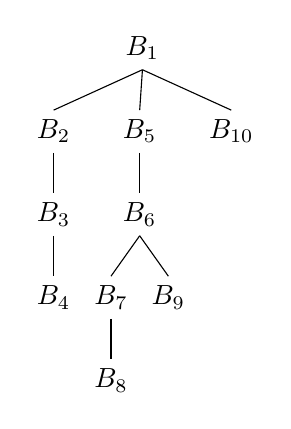
\begin{tikzpicture}
        \Tree
            [.$B_1$
                [.$B_2$ [.$B_3$ $B_4$ ] ]
                [.$B_5$ [.$B_6$ [.$B_7$ $B_8$ ] $B_9$ ] ]
                $B_{10}$
            ]
    \end{tikzpicture}

    \caption{
        The dominator tree for the control flow graph in figure \ref{fig:cfg}.
    }
    \label{fig:dominator-tree}
\end{figure}

\begin{figure}[ht]
    \centering
    \begin{tabular}{|r|p{13cm}|}
        \hline \\
        \textbf{Line number} & \textbf{Reaching definitions} \\ \hline
        $5$ : & $\{(n, 1), (m, 2), (x, 3), (y, 4)\}$ \\ \hline
        $7$ : & $\{(n, 1), (m, 2), (x, 3), (y, 4)\}$ \\ \hline
        $8$ : & $\{
            (n, 1), (m, 2), (x, 3), (y, 4), (s, 6), (t_1, 8), (t_2, 9),
            (t_3, 10), (n, 11)\}$ \\ \hline
        $12$ : & $\{
            (m, 2), (x, 3), (y, 4), (s, 6), (t_1, 8), (t_2, 9), (t_3, 10),
            (n, 11)\}$ \\ \hline
        $16$ : & $\{(n, 1), (m, 2), (x, 3), (y, 4)\}$ \\ \hline
        $18$ : & $\{
            (n, 1), (m, 2), (x, 3), (y, 4), (p, 16), (i, 17)\}$ \\ \hline
        $24$ : & $\{
            (n, 1), (m, 2), (x, 3), (y, 4), (p, 16), (i, 17), (p, 25), (i, 17),
            (i, 26), (t_1, 20), (t_2, 22)\}$ \\ \hline
        $28$ : & $\{
            (n, 1), (m, 2), (x, 3), (y, 4), (p, 16), (i, 17), (p, 25), (i, 17),
            (i, 26), (t_1, 20), (t_2, 22)\}$ \\ \hline
        $30$ : & $\{
            (n, 1), (m, 2), (x, 3), (y, 4), (s, 6), (t_1, 8), (t_2, 9),
            (t_3, 10), (n, 11)\}$ \linebreak $\cup \{
            (p, 16), (i, 17), (p, 25), (i, 26), (t_1, 20), (t_2, 22)\}$ \\
        \hline
    \end{tabular}

    \caption{The reaching definition at various points in the program.}
    \label{fig:reaching-defs}
\end{figure}

Figure \ref{fig:reaching-defs} shows the reaching definitions in the program.
Based on this analysis, there are some optimizations that we can perform.
\begin{itemize}
    \item On line $8$, we compute $t_1 \gets x \times y$, but the reaching
        definitions of $x$ and $y$ are outside the loop. Hence, we can hoist
        this computation outside the loop; it is a loop invariant.

    \item Now we notice that $t_2 \gets \mathtt{sum}(t_1)$ has become a loop
        invariant, so we may hoist it out as well.

    \item Likewise, $t_3 \gets s + t_2$ has become loop-invariant, so we may
        hoist it out.

    \item On line $22$, $t_2 \gets \mathtt{sum}(x_{tr})$ is loop-invariant, so
        we may hoist it out.

    \item Since the check $t_2 < 0$ on line $22$ is loop-invariant, it might be
        possible to hoist the entire \texttt{if}-statement out of the loop, and
        refactor so that the loop is only executed if $t_2 \geq 0$. However,
        since the program is dynamically typed, this might actually alter the
        semantics of the program: lines $20$, $21$, and $22$ could crash the
        program due to type errors, but this loop code motion could cause those
        lines to never be executed now.
\end{itemize}

\subsection{Superlive variables}

\begin{description}
    \item[Approximation.] Sets of variables.

    \item[Precise definition.]
        A variable $x$ is said to be \emph{superlive} at a program point $p$ if
        on \emph{all} paths from $p$ to the end of the program, the value of
        the variable $x$ is used.

    \item[Analysis direction.]
        This is a backwards analysis, because we want to obtain information
        ``about the future''.

    \item[Merge operator.]
        Because this is a \emph{must} analysis (on ``all'' paths, a property
        must hold), we merge information using set intersection $\cap$.

    \item[Dataflow equation.]
        Since this is a backwards analysis, we must compute for a statement
        $S$, given its output $\Out{S}$, its input $\In{S}$.
        \begin{equation*}
            \In{S} = \left(\Out{S} \setminus \Kill{S}\right) \cup \Gen{S}
        \end{equation*}
        where
        \begin{itemize}
            \item $\Kill{S}$ is the set of all variables written to in the
                statement $S$.

            \item $\Gen{S}$ is the set of all variables being read in the
                statement $S$.
        \end{itemize}

        We kill then union the gen set because of situations like $x = x + 1$.
        Here, $x$ must be considered superlive before this statement, since its
        value is being read by the statement. If we killed after performing the
        union with the gen set, then $x$ would not appear in $\In{S}$, and the
        analysis would be incorrect.

    \item[Initial conditions.]
        \begin{align*}
            \In{\mathtt{END}} &= \emptyset \\
            \In{S_i} &= \emptyset
        \end{align*}
\end{description}

\subsection{The joy of dynamic typing}

The program in figure \ref{fig:dynamic-1} demonstrates the dynamic typing of
the language we are studying.

\begin{figure}[ht]
    \begin{lstlisting}
read_int(z);
if(z < 0) {
    y = int(3);
}
else {
    y = 3.5;
}
x = y;
    \end{lstlisting}

    \caption{A simple program fragment that demonstrates dynamic typing.}
    \label{fig:dynamic-1}
\end{figure}

The program in figure \ref{fig:dynamic-2} demonstrates another instance of
dynamic typing, but in which at least one program path leads to an error.

\begin{figure}[ht]
    \begin{lstlisting}
read_int(z);
if(z < 0) {
    y = [1,2,3];
}
else {
    y = 3;
}
while(1) {
    x = transpose(y);
}
    \end{lstlisting}

    \caption{
        A simple program fragment that demonstrates a situation in which errors
        can arise due to dynamic typing. The statement involving
        \texttt{transpose} will raise a runtime error if the \texttt{else}
        branch of the \texttt{if}-statement is taken during execution.
    }
    \label{fig:dynamic-2}
\end{figure}

We will define a static analysis to estimate the possible types for a variable.

\begin{description}
    \item[Approximation.]
        Sets of pairs, associating variables with types.

        For example, the pair $(x, \intty)$ indicates that the
        variable $x$ has the type \texttt{int} as a possible type. The set
        $\{(x, \intty), (x, \doublety)\}$ indicates that the variable $x$ is an
        integer or a double.

    \item[Precise definition.]
        A variable $x$ is said to have approximate type $t$ at a program point
        $p$ if there exists a path $P$ to point $p$ from an assignment to $x$
        with inferred type $t$ along which no other assignment to $x$ is made.

    \item[Analysis direction.]
        Since we are looking into the past, (what assignments have been made to
        $x$ up till now?) this is forwards analysis.

    \item[Merge operator.]
        Since this is a \emph{may} analysis, (the precise definition used the
        wording ``there exists a path'',) the merge operator is set union
        $\cup$.

    \item[Dataflow equation.]
        This is a forwards analysis, so we must compute $\Out{S}$ given
        $\In{S}$.
        \begin{equation*}
            \Out{S} = \left(\In{S} \setminus \Kill{S}\right) \cup \Gen{S}
        \end{equation*}
        where
        \begin{itemize}
            \item $\Gen{S}$ is the set of all assignments in the statement $S$
                along with their inferred types.

            \item $\Kill{S}$ is the set of all pairs $(x, t)$ where $x$ is a
                variable being written to in $S$, and $t$ is arbitrary.
        \end{itemize}

        The intuition for these choices comes from analyzing a statement like
        $x \gets y$. The analysis should proceed by:
        \begin{enumerate}
            \item inferring the type(s) of $y$, which may involving using
                knowledge of the known types of $x$;
            \item discarding all known typing information for $x$;
            \item storing the inferred type(s) of $y$ as types for $x$.
        \end{enumerate}

    \item[Initial conditions.]
        \begin{align*}
            \In{\mathtt{START}} &= \emptyset \\
            \In{S_i} &= \emptyset
        \end{align*}
\end{description}

\begin{figure}[ht]
    \centering
    \begin{lstlisting}
read_int(z); // (z, int)
if(z < 0) {
    y = int(3); // (y, int)
}
else {
    y = 3.5; // (y, double)
}
x = y; // (y, int), (y, double)
    \end{lstlisting}

    \caption{
        The program fragment given in \ref{fig:dynamic-1}, but annotated with
        the result of our analysis.
    }
    \label{fig:ann-dynamic-1}
\end{figure}

\begin{figure}[ht]
    \centering
    \begin{lstlisting}
read_int(z);
if(z < 0) {
    y = [1,2,3]; // (y, array)
}
else {
    y = int(3); // (y, int)
}
while(1) {
    x = transpose(y); // (y, int), (y, array), (x, array)
}
    \end{lstlisting}

    \caption{
        The program fragment given in \ref{fig:dynamic-2}, but annotated with
        the result of our analysis.
    }
    \label{fig:ann-dynamic-2}
\end{figure}

Figures \ref{fig:ann-dynamic-1} and \ref{fig:ann-dynamic-2} show the results of
our analysis on the two program fragments we wrote.

This type approximation analysis can be used for generating warnings when a
program path might lead to a type error, such as in figure
\ref{fig:ann-dynamic-2}. It can also be used to avoid runtime type checks in
JIT-compiled code. \texttt{transpose} requires its argument to be an array, so
it must check this at runtime in general; if we can prove that along all paths,
its argument is in fact an array, then we can replace the call to
\texttt{transpose} with a call to \texttt{unsafe\_transpose} that does not
perform the check, and is consequently faster. (I believe a similar
optimization exists in Java, where array bounds-checking is skipped if the
JIT-compiler can guarantee than the index is within the array bounds.)

\end{document}
